\documentclass{standalone}
\usepackage{tikz}
\usetikzlibrary{shapes,decorations, positioning}

\begin{document}
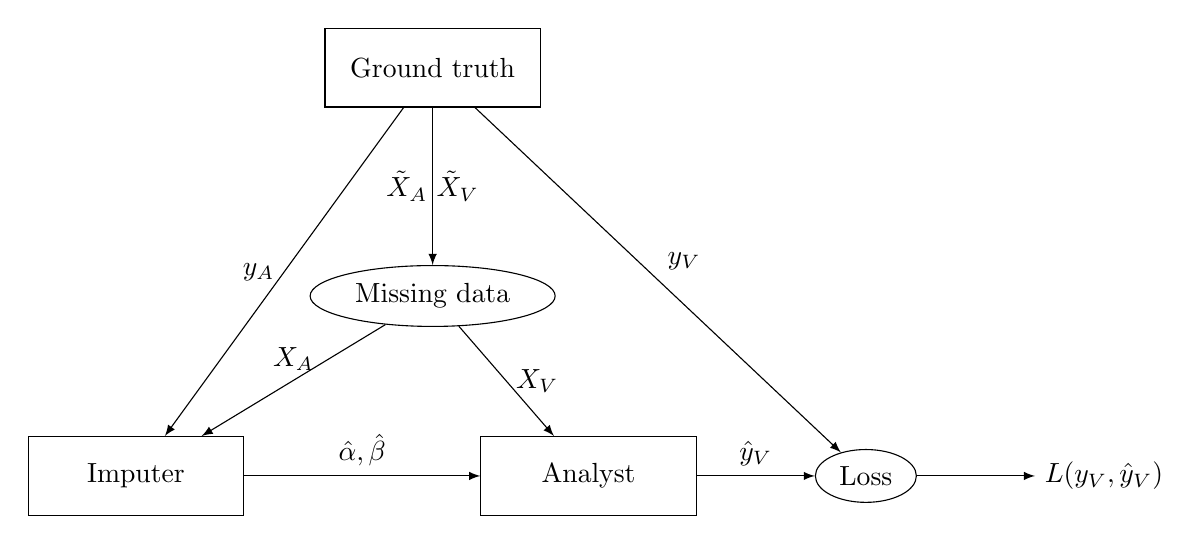
\begin{tikzpicture}[
node distance=1.5cm and 1.5cm,
ar/.style={->,>=latex},
mynode/.style={
  draw,
  text width=2.5cm,
  minimum height=1cm,
  align=center
  }
]
  \node[mynode] (imp) {Imputer};
  \node[mynode,right=3cm of imp] (an) {Analyst};
  \node[ellipse,draw,above left=1.5cm and -0.5cm of an] (md) {Missing data};
  \node[mynode,above=2cm of md] (gt) {Ground truth};
  \node[ellipse,draw,right=of an] (loss) {Loss};
  \node[right=of loss] (res) {$L(y_V, \hat{y}_V)$};
  
  \draw[ar] 
  (gt) -- node {$\tilde{X}_A\ \tilde{X}_V$} (md);
  \draw[ar] 
  (gt) -- node[left] {$y_A$} (imp);
  \draw[ar] 
  (gt) -- node[above,auto] {$y_V$} (loss);
  \draw[ar] 
  (md) -- node[above] {$X_A$} (imp);
  \draw[ar] 
  (md) -- node[right] {$X_V$} (an);
  \draw[ar] 
  (imp) -- node[left,auto] {$\hat{\alpha}, \hat{\beta}$} (an);
  \draw[ar] 
  (an) -- node[above,auto] {$\hat{y}_V$} (loss);
  \draw[ar] 
  (loss) -- node[left,auto] {} (res);
\end{tikzpicture}
\end{document}